In diesem Kapitel wird erklärt was die Motivation, die Problemstellung und die Methode die zur Ausarbeitung verwendet wurde. Abschließend wird der grobe Aufbau und der rote Faden dieser Arbeit beschrieben. 

\section{Motivation}

Landwirtschaft spielt für jede Gesellschaft eine entscheidende Rolle, da ohne sie die Ernährung der Bürger unmöglich wäre. Für einen Staat ist eine moderne und effiziente Landwirtschaft wichtig um Abhängigkeiten zu anderen Staaten zu verhindern oder zumindest zu verringern. Daher ist dieses Thema auch für Länder der ersten Welt auf der Agenda. Da die Personalkosten hoch sind, ist die Effizienzsteigerung durch Technologie entscheidend für die Entwicklung des Landwirtschaftssektor.

Durch den ständig steigenden Energiebedarf ist vor allem die Frage nach eines optimalen Einsatzes von Energie wichtig für Zukunft der Landwirtschaftsbetriebe in der EU. Neben der Forschung in den Disziplinen der Chemie und des Maschinenbaus, ist die Informatik eine interessante Quelle für kleine und große Optimierungen des landwirtschaftlichen Betriebs. Da ich den Blick über den Tellerrand nicht nur nicht scheue sondern gerne wage und aus einem landwirtschaftlich genutzten Gebiet in Niederösterreich, dem Marchfeld, stamme, liegt mir die Zukunft der Landwirtschaft in Europa am Herzen.

\section{Problemstellung}

Diese Arbeit beschäftigt sich mit der Ausarbeitung des aktuellen Standes der Steigerung der Energieeffizienz in der Landwirtschaft mittels ICTs (Informations- und Kommunikationstechnik). Dazu wird ein nicht vollständiger Überblick der Literatur der letzten 4 Jahre zu dem Themen Energieeffizienz in der Landwirtschaft erstellt. Der Fokus ist eine Übersicht über Sensorsysteme, Planungssysteme und Unterstützungssysteme. Als Basis werden Arbeiten zur Modellierung der notwendigen Informationsbasis vorgestellt.

\section{Verwendete Methode}

Die Quellen für diese Arbeit wurden ohne Fokus auf bestimmte Konferenzen oder Datenbanken ausgewählt. 

\subsection{Literaturrecherche}
Um keine relevanten Arbeiten zu übersehen wurden neben den akademischen Datenbanken und Bibliotheken werden Berichte von relevanten Forschungsgruppen der EU herangezogen. Für die Suche nach Literatur wurden verschiedene Kombinationen aus folgenden Suchbegriffen gewählt:

\textit{energy, efficency, it, informatic, stochastic, agriculture, Landwirtschaft, Effizenz, ICT, Informationstechnologie, Planung, precision farming, planning, DSS, decision support system, GIS, geo information system}

\subsection{Selektionsvorgang}
Die wissenschaftliche Literatur wurde auf Basis folgender Kriterien bewertet:
\begin{itemize}
  \item Energieeffizenzrelevanz. Bei der Suche muss das Thema direkt oder indirekt zur Steigerung der Energieeffizenz beitragen. Dazu zählen sowohl Aufwand von Wasser wie Auslastung von vorhandenen Landwirtschaftsmaschinen.
  \item ICT-Relevanz. Bei der Suche nach Effizienz in der Landwirtschaft mussten alle Themen aussortiert werden die sich auf Effizienzsteigerung durch chemische Präparate oder bestimmte Entwicklungen im Maschinenbau bezogen.
  \item Veröffentlichungsmedium. Arbeiten die weder im Rahmen einer Konferenz noch in einem Journals oder zu in einem wissenschaftlichen Magazins veröffentlicht wurden, wurden aussortiert.
  \item Aktualität. Die Arbeiten mussten relativ aktuell sein. Werke die vor 2010 geschrieben wurden, wurden nicht weiter verfolgt, mit Ausnahme von Literatur die nötige Grundlagen erläutert.
\end{itemize}

\section{Verwandte Arbeiten}
Das Interesse in eine effiziente Landwirtschaft durch den Einsatz von ICTs wird in \cite{jour:Andreopoulou2012} vorgestellt, auch wenn der Fokus auf Nachhaltigkeit liegt. Effizienz ist dabei Mittel zum Zweck. Durch verschiedene Förderungen versucht die EU dies voranzutreiben. Eine Übersicht der verschiedenen Forschungsrichtungen wird im Bericht des Projekts \cite{misc:Mikkola2013} geboten. Eine mögliche Stoßrichtung um hohe Effizienz in der Aufzucht von Pflanzen zu erreichen ist \textit{Precision Farming}\cite{jour:Auernhammer2001}.

Die vorgeschlagenen Forschungsschwerpunkte \textit{Sensor technology} wird von den Arbeiten von Zhou Jianjun, Wang Xiaofang, Wang Xiu, Zou Wei und Cai Jichen in \cite{proc:Zhou2013} aufgegriffen. Für Sensoren in Glashäusern haben Mancuso und Bustaffa eine Studie\cite{misc:Mancuso2006} präsentiert die zeigt wie Sensoren Mikroklimas messen und Pilzerkrankungen verhindern können. Kontextsensitive Landwirtschaftsorganisationssysteme die auf Sensornetzwerken aufbauen werden in \cite{proc:Khaydarov2012} behandelt. Eine Möglichkeit wie diese Daten kostengünstig in einem automatisiertem System behandelt werden können, wird in \cite{jour:Kamalesh2014} vorgestellt. In \cite{jour:Shaikh2010} wird ein Framework vorgestellt wie 	kontextsensitive Grid-Systeme gebaut werden können.

Neben \textit{Sensor technology} wird die Forschung betreffend \textit{Design Tools} und \textit{Decision Support Systems} angeregt. Ein Vorschlag wie ein solche Planungsprogramme entwickelt werden könnten, wird in \cite{art:Wang2011} vorgeschlagen. Ein Ansatz der GIS-Systeme, Webtechnologie und Data-Mining vereint um ein Expertensystem das verschiedene Bedürfnisse verschiedener Länder beachten kann, wird in \cite{jour:Zhu2009} vorgestellt. Auf die Frage wie solche Daten modelliert werden können, wird in \cite{jour:Schulze2007} behandelt. \cite{jour:Aqeel-ur-Rehman2011} beschäftigt sich mit dem weiterführenden Thema wie Umwelteinflüsse auf den Ertrag modelliert werden können.

Mögliche Hürden die eine Adaption ICT-Lösungen von Landwirtschaftstreibenden und wie diese überwunden werden können, wird in \cite{jour:Aubert2012} vorgestellt.

\section{Abgrenzung}
Diese Arbeit ist durch die zeitliche Beschränkung im Umfang beschränkt. Deshalb konzentriert sich diese Arbeit auf die in \cite{misc:Mikkola2013} als wichtigsten Themen genannten Punkte:

\begin{itemize}
	\item Sensorsysteme (GIS- und Sensornetzwerksysteme)
	\item Datenmodellierung
	\item Entscheidungsunterstützungssysteme und artverwandte Planungsanwendungen.
\end{itemize}

Ziel der Arbeit ist es einen Überblick über Arbeiten in diesem Gebiet zu geben. Es ist nicht das Ziel neue Erkenntnisse durch Forschung hinzuzufügen oder einen umfassenden Überblick über alle wichtigen Themen für die Steigerung der Energieeffizienz in der Landwirtschaft zu geben.

\section{Aufbau der Arbeit}

Optimierungen jeder Art laufen in einem iterativen Prozess ab. Ein jeder Schritt besteht aus folgenden Tätigkeiten: 

\begin{itemize}
	\item Aktuelle Kennzahlen messen.
	\item Optimierungen durchführen.
	\item Erfolg der Optimierung messen.
\end{itemize}

Diese Schritte werden solange wiederholt bis ein zufriedenstellendes Ergebnis erreicht wird. Im Bereich der Energieeffizienz in der Landwirtschaft spielen hier mehrere Teilkomponenten zusammen. Abbildung \ref{fig:topic_overview} zeigt die Themen die hier behandelt werden und wie diese in Beziehung stehen.

\begin{figure}[h]
 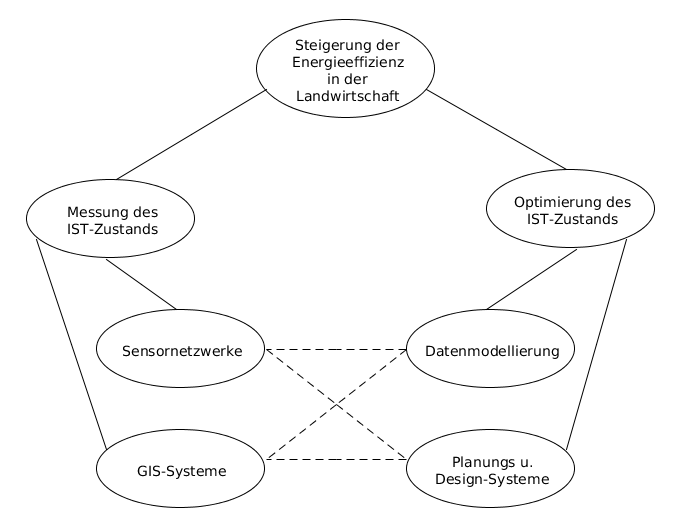
\includegraphics[scale=0.65,natwidth=\textwidth]{figures/introduction/topic_overview.png}
 \centering
 \label{fig:topic_overview}
 \caption{Beziehungen zwischen Themen der Arbeit. Schwarze Linien verbinden Thmen mit Unterpunkten und gestrichelte Linien verbinden Themen die in Beziehung stehen.}
\end{figure}

Die Steigerung der Effizienz durch ICTs basiert darauf, dass die Messung von relevanten Kennzahlen zeitnah und schnell durchgeführt werden können und die Optimierung der betreffenden Stellen rechnergestützt oder automatisch geschehen.

Diese Arbeit behandelt die Bedeutung von Sensornetzwerken und GIS-Systeme und wie diese mit Planungssystemen zusammen hängen. Damit Messdaten ausgewertet werden können müssen diese als Eingabewerte modelliert werden. 

Die Modellierung geschieht innerhalb der Applikation und als Optimierungsproblem. Die Basis für die Behandlung des mathematischen Effizienzproblems stellen zwei Modellierungsklassen:

\begin{itemize}
	\item DEA (Data Envelopment Analysis)
	\item SFA (Stochastische Frontier Analyse)
\end{itemize}

Aufbauend auf diesen Modellierungsklassen werden Arbeiten vorgestellt die für Landwirtschaftseffizienzsteigerung geschrieben wurden.

Die Daten aus den mathematischen Optimierungsmodellen und der GIS- und lokalen Sensorsystemen werde von Planungs-Software verwendet. Diese Planungssysteme unterteilen sich in automatische Steuerungssysteme und semi-automatische Entscheidunghilfen sowie Planungsanwendungen. 

Die Kapitel stellen exemplarisch Arbeiten vor um so einen Überblick über die aktuelle Forschung zu geben.